%-- einleitung
\section{Konzept}
In diesem Abschnitt werden die konzeptionellen Planungen des Projekts mithilfe einer Anforderungsanalyse und einer Systemmodellierung dargestellt.

\subsection{Anforderungsanalyse}
In der Tabelle \ref{tab:fa} sind die funktionalen Anforderungen aufgelistet. Diese beschreiben, was in diesem Projekt alles umgesetzt werden muss. Die funktionale Anforderung 1FA gibt vor, dass die benötigten Daten zum Berechnen des TSP dynamisch ausgelesen werden sollen. Damit soll verhindert werden, dass die Daten als Teil des Programmcodes, hart programmiert, gespeichert werden.
In der funktionalen Anforderung 2FA wird vorgegeben, dass das System das TSP mit Genetischen Algorithmen lösen soll. In der Anforderung 3FA wird beschrieben, wie die Routen des TSP zu Bewerten sind.\\
In der Tabelle \ref{tab:nfa} sind die nichtfunktionalen Anforderungen aufgelistet. Diese beschreiben, wie das Projekt umgesetzt werden soll. In der nichtfunktionalen Anforderung 1NFA wird das Laufzeitsystem vorgegeben. Die Anforderungen 2NFA, 3NFA und 4NFA geben Qualitätsvorgaben vor. Die nichtfunktionale Anforderung 5NFA besagt, dass am Ende der Entwicklung ein ausführbares Programm vorliegen muss.

\begin{table}[H]
\caption{Funktionalen Anforderungen}
\begin{tabular}{|c|p{12.5cm}|}
Nummer & Beschreibung \\
\hline
1FA & Die Liste der Städte (Namen + Distanzen) sollen aus einer Datei (mit bestimmter Formatierung) auslesbar sein, damit diese Daten ohne Programmieraufwand verändert werden können. \\  
2FA & Das System soll mit Genetischen Algorithmen das Travelling Salesman Problem umsetzen. \\  
3FA & Das System soll Routen auf Grundlage derer Gesamtdistanz beurteilen und weiterverarbeiten. \\  
\end{tabular}
\label{tab:fa}
\end{table}
\begin{table}[H]
\caption{Nichtfunktionalen Anforderungen}
\begin{tabular}{|c|p{12.5cm}|}
 Nummer & Beschreibung \\ 
\hline
1NFA & Das System soll auf Windows 10 ausführbar sein.\\
2NFA & Das System soll vollständig dokumentiert sein.\\
3NFA & Das System soll leicht testbar sein.\\
4NFA & Das System soll leicht bedienbar sein.\\
5NFA & Das System soll als Executable ausführbar sein.\\
\end{tabular}
\label{tab:nfa}
\end{table}

\subsection{Systemmodellierung}
In Abbildung \ref{fig:systemmodellierung} ist ein FMC-Diagramm zu sehen, das eine Übersicht über die Projektarchitektur bietet.
Die Genetischen Algorithmen werden innerhalb einer eigenen Bibliothek implementiert. Das hat den Vorteil, dass das System durch eine solche Architektur eine hohe Wiederverwendbarkeit aufweist. Darüber hinaus ergibt sich dadurch eine klare Trennung von einem Frontend zu der Bibliothek.
Innerhalb der Bibliothek verbirgt ein Simulator die Komplexität der eigentlichen Genetischen Algorithmen. Über den Simulator können Parametereinstellungen vorgenommen werden, die den Ablauf der Vorgänge steuern.
Der Simulator verwendet die Genetischen Algorithmen über einheitliche Schnittstellen, über die entweder Populationen oder Individuen ausgetauscht werden. Dadurch ist das System leicht bedienbar, was die Anforderung 4NFA erfüllt. Darüber hinaus ermöglicht diese klare Architektur eine leichte Testbarkeit und erfüllt die Anforderung 3NFA. Die Library soll über ein Frontend ausgeführt werden und somit dem Benutzer die Möglichkeit geben einfach Simulationen durchzuführen. Dieses Projekt beschäftigt sich allerdings vornehmlich mit der Entwicklung der Bibliothek und weniger mit der Entwicklung des Frontends.

\begin{figure}[H]
\centering
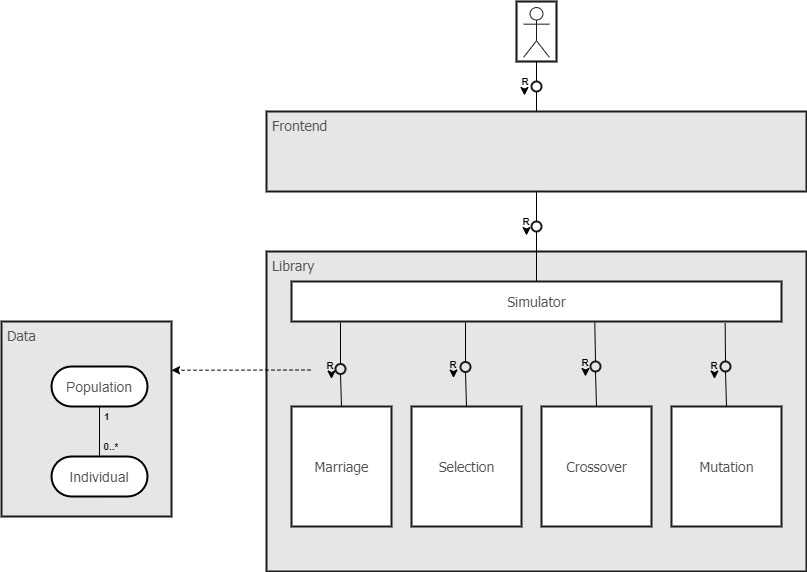
\includegraphics[width=1\textwidth]{img/Vortrag/Systemmodellierung.png}
\caption{Systemmodellierung}
\label{fig:systemmodellierung}
\end{figure}

%--